\section{Komplexe Funktion, Abbildungen}
	\begin{minipage}[t]{0.5\textwidth}
		\subsection{Definition}
			\hfill\\
			\scalebox{0.5}{\begin{tikzpicture}
	\node[black!70!green] at (0.5, 5.7) {$z_1$};
	\node[black!70!green] at (0.5, 5) {$z_2$};
	\draw[->, black!70!green, very thick] (0.7, 5.7) -- (1, 5.4);
	\draw[->, black!70!green, very thick] (0.7, 5) -- (1, 5.3);
	\node[black!70!green] at (2.3, 5.35) {$z = z_1 + \mathrm{j} z_2$};
	\draw[->, black!70!green, very thick] (3.5, 5.35) -- (7, 5.35);
	
	\node[blue] at (16, 5.7) {$w_1$};
	\node[blue] at (16, 5) {$w_2$};
	\draw[->, blue, very thick] (15.3, 5.4) -- (15.6, 5.7);
	\draw[->, blue, very thick] (15.3, 5.3) -- (15.6, 5);
	\node[blue] at (14, 5.35) {$w = w_1 + \mathrm{j} w_2$};
	\draw[->, blue, very thick] (9.5, 5.35) -- (12.5, 5.35);
	
	\node[minimum size=2cm, draw] at (8.3, 5.35) {\scalebox{3}{$\textcolor{red}{f}$}};
	
	\draw[->, very thick, red] (22:8cm) arc[radius=1, start angle=140, end angle=40] node[above, red] at (8.3, 3.3) {$f$};
	\node[above, red] at (8.3, 3.8) {$z \rightarrowtail w = f(z)$};
	
	\node[above, font=\large\bfseries] at (1, 5.8) {$\underline{\text{z-Ebene:}}$};
	\begin{tikzpicture}
	\begin{axis}[
		axis lines=middle,
		axis equal,
		xmin=-2,
		xmax=2,
		ymin=-2,
		ymax=2,
		xlabel=$z_1$,
		ylabel=$z_2$,
		xticklabels={,,},
		yticklabels={,,}
	]
		\addplot[draw=none] coordinates {(1, 1)};
		\addplot[mark=*, black!70!green] coordinates {(-0.5, 0.5)} node[below, black!70!green] {$z$} node[above, black!70!green] {Orginalpunkt};
		\node at (axis cs:1.5, 1) {\scalebox{2.5}{\rom{1}}};
		\node at (axis cs:-1.5, 1) {\scalebox{2.5}{\rom{2}}};
		\node at (axis cs:-1.5, -1) {\scalebox{2.5}{\rom{3}}};
		\node at (axis cs:1.5, -1) {\scalebox{2.5}{\rom{4}}};
	\end{axis}
\end{tikzpicture}\hspace{2.7cm}%
	
	\node[above, font=\large\bfseries] at (1.2, 5.8) {$\underline{\text{w-Ebene:}}$};
	\begin{tikzpicture}
	\begin{axis}[
		axis lines=middle,
		axis equal,
		xmin=-2,
		xmax=2,
		ymin=-2,
		ymax=2,
		xlabel=$w_1$,
		ylabel=$w_2$,
		xticklabels={,,},
		yticklabels={,,}
	]
		\addplot[draw=none] coordinates {(1,1)};
		\addplot[mark=*, blue] coordinates {(0.5, -0.5)} node[below, blue] {$w$} node[above, blue] {Bildpunkt};
		\node at (axis cs:1.5, 1) {\scalebox{2.5}{\rom{1}}};
		\node at (axis cs:-1.5, 1) {\scalebox{2.5}{\rom{2}}};
		\node at (axis cs:-1.5, -1) {\scalebox{2.5}{\rom{3}}};
		\node at (axis cs:1.5, -1) {\scalebox{2.5}{\rom{4}}};
	\end{axis}
\end{tikzpicture}
\end{tikzpicture}}
	\end{minipage}
	\begin{minipage}[t]{0.5\textwidth}
		\subsection{Winkeltreue}
			Komplexe Funktion $f\left( z \right)$ ist in allen Punkten winkeltreu, wo gibt: \fbox{$f^{\prime}\left( z \right) \neq 0$}\\[6pt]
			Sie bewirkt \textbf{lokal eine Drehstreckung:}\\[3pt]
			\begin{tabular}{ll}
				Streckungsfaktor: & \fbox{$\left|f^{\prime}(z)\right|$}\\[3pt]
				Drehwinkel: & \fbox{$\operatorname{\arg}\left( z \right)$}\\[3pt]
				Verschieben: & \fbox{$f^{\prime}\left( z \right)$}
			\end{tabular}
	\end{minipage}

\subsection{Parameter- und Koordinatengleichung}
	\begin{minipage}[]{0.2\textwidth}
		\scalebox{0.5}{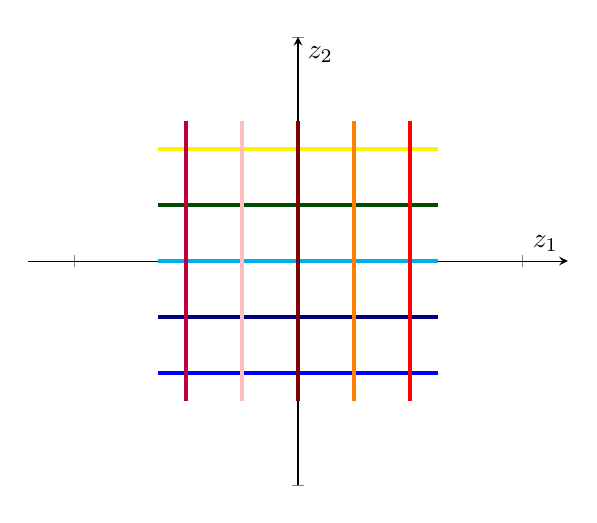
\begin{tikzpicture}
	\begin{axis}[
		axis lines=middle,
		axis equal,
		xmin=-4,
		xmax=4,
		ymin=-4,
		ymax=4,
		xlabel=$z_1$,
		ylabel=$z_2$,
		xticklabels={,,},
		yticklabels={,,}
	]
		\addplot[-, yellow, ultra thick] coordinates {(-2.5, 2) (2.5, 2)};
		\addplot[-, black!70!green, ultra thick] coordinates {(-2.5, 1) (2.5, 1)};
		\addplot[-, cyan, ultra thick] coordinates {(-2.5, 0) (2.5, 0)};
		\addplot[-, black!50!blue, ultra thick] coordinates {(-2.5, -1) (2.5, -1)};
		\addplot[-, blue, ultra thick] coordinates {(-2.5, -2) (2.5, -2)};
		
		\addplot[-, purple, ultra thick] coordinates {(-2, -2.5) (-2, 2.5)};
		\addplot[-, pink, ultra thick] coordinates {(-1, -2.5) (-1, 2.5)};
		\addplot[-, black!50!red, ultra thick] coordinates {(0, -2.5) (0, 2.5)};
		\addplot[-, orange, ultra thick] coordinates {(1, -2.5) (1, 2.5)};
		\addplot[-, red, ultra thick] coordinates {(2, -2.5) (2, 2.5)};
	\end{axis}
\end{tikzpicture}}
	\end{minipage}
	\begin{minipage}[]{0.8\textwidth}
		\begin{tabular}{llll}
			\textbf{waagrechte Gitternetzlinien durch Punkt $(0; c_2)$:} & &\\[3pt]
		\end{tabular}
		\begin{tabular}{llll}
			\fbox{$z = \operatorname{z}\left( r \right) = r + \mathrm{j} c_2$} & $\xrightarrow[]{f\left( z \right)}$ & \fbox{$w = \operatorname{w}\left( r \right) = f\left( \operatorname{z}\left( r \right) \right) = f\left( r + \mathrm{j} c_2 \right)$} & mit $r \subset \mathbb{R}$\\[3pt]
		\end{tabular}
		\begin{tabular}{llll}
			\textbf{senkrechte Gitternetzlinien durch Punkt $(c_1; 0)$:} & & &\\[3pt]
		\end{tabular}
		\begin{tabular}{llll}
			\fbox{$z = \operatorname{z}\left( r \right) = c_1 + \mathrm{j} r$} & $\xrightarrow[]{f\left( z \right)}$ & \fbox{$w = \operatorname{w}\left( r \right) = f\left( \operatorname{z}\left( r \right) \right) = f\left( c_1 + \mathrm{j} r \right)$} & mit $r \subset \mathbb{R}$\\[3pt]
		\end{tabular}
		\begin{tabular}{llll}
			\textbf{Koordinatengleichung:} & 
			\fbox{$\left| \begin{array}{c}
				w_1 = \operatorname{Re}\left(\left[ f\left(\operatorname{z}\left(r \right)\right)\right]\right)\\[3pt]
				w_2 = \operatorname{Re}\left(\left[ f\left(\operatorname{z}\left(r \right)\right)\right]\right)
				\end{array} \right|$} &
			$\Rightarrow$ & 
			$\begin{array}{l}
				\text{Parameter $r$ eliminieren,}\\[3pt]
				\text{um Koordinatengleichung}\\[3pt]
				\text{zu erhalten.}
			\end{array}$
		\end{tabular}
	\end{minipage}

\subsection{Lineare Funktion}
	\begin{minipage}[]{0.5\textwidth}
		\scalebox{0.5}{\begin{tikzpicture}	
	\draw[->, very thick, red] (22:8cm) arc[radius=1, start angle=140, end angle=40] node[above, red] at (8.3, 3.3) {$z \rightarrowtail w = f(z)$} node at (8.3, 2.3) {$f(z) = a \cdot z + b$};
	
	\begin{tikzpicture}
	\begin{axis}[
		axis lines=middle,
		axis equal,
		xmin=-4,
		xmax=4,
		ymin=-4,
		ymax=4,
		xlabel=$z_1$,
		ylabel=$z_2$,
		xticklabels={,,},
		yticklabels={,,}
	]
		\addplot[-, yellow, ultra thick] coordinates {(-2.5, 2) (2.5, 2)};
		\addplot[-, black!70!green, ultra thick] coordinates {(-2.5, 1) (2.5, 1)};
		\addplot[-, cyan, ultra thick] coordinates {(-2.5, 0) (2.5, 0)};
		\addplot[-, black!50!blue, ultra thick] coordinates {(-2.5, -1) (2.5, -1)};
		\addplot[-, blue, ultra thick] coordinates {(-2.5, -2) (2.5, -2)};
		
		\addplot[-, purple, ultra thick] coordinates {(-2, -2.5) (-2, 2.5)};
		\addplot[-, pink, ultra thick] coordinates {(-1, -2.5) (-1, 2.5)};
		\addplot[-, black!50!red, ultra thick] coordinates {(0, -2.5) (0, 2.5)};
		\addplot[-, orange, ultra thick] coordinates {(1, -2.5) (1, 2.5)};
		\addplot[-, red, ultra thick] coordinates {(2, -2.5) (2, 2.5)};
	\end{axis}
\end{tikzpicture}\hspace{2.7cm}%
	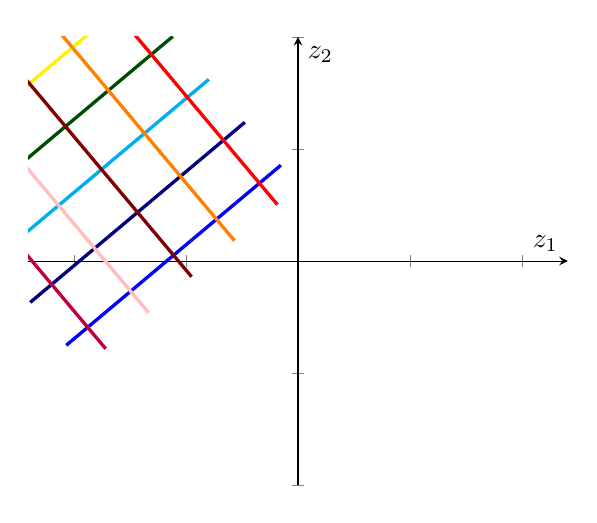
\begin{tikzpicture}
	\begin{axis}[
		axis lines=middle,
		axis equal,
		xmin=-4,
		xmax=4,
		ymin=-4,
		ymax=4,
		xlabel=$z_1$,
		ylabel=$z_2$,
		xticklabels={,,},
		yticklabels={,,}
	]
		\addplot[-, yellow, very thick, rotate=40] coordinates {(-2.5, 2) (2.5, 2)};
		\addplot[-, black!70!green, very thick, rotate=40] coordinates {(-2.5, 1) (2.5, 1)};
		\addplot[-, cyan, very thick, rotate=40] coordinates {(-2.5, 0) (2.5, 0)};
		\addplot[-, black!50!blue, very thick, rotate=40] coordinates {(-2.5, -1) (2.5, -1)};
		\addplot[-, blue, very thick, rotate=40] coordinates {(-2.5, -2) (2.5, -2)};
		
		\addplot[-, purple, very thick, rotate=40] coordinates {(-2, -2.5) (-2, 2.5)};
		\addplot[-, pink, very thick, rotate=40] coordinates {(-1, -2.5) (-1, 2.5)};
		\addplot[-, black!50!red, very thick, rotate=40] coordinates {(0, -2.5) (0, 2.5)};
		\addplot[-, orange, very thick, rotate=40] coordinates {(1, -2.5) (1, 2.5)};
		\addplot[-, red, very thick, rotate=40] coordinates {(2, -2.5) (2, 2.5)};
	\end{axis}
\end{tikzpicture}
\end{tikzpicture}}
	\end{minipage}
	\begin{minipage}[]{0.5\textwidth}
		Die lineare Funktion $w = f\left( z \right) = a z + b$ bewirkt:\\[3pt]
		\renewcommand{\arraystretch}{1.7}
		\begin{tabular}{|lll|}
			\hline
			Drehstreckung mit: & Streckungsfaktor & $\left|a\right|$\\
	 & Drehwinkel & $\operatorname{arg}\left( a \right)$\\
	 & Zentrum & $\dfrac{b}{1-a}$\\[6pt]
			\hline
			Drehstreckung mit: & Streckungsfaktor & $\left|a\right|$\\
			& Drehwinkel & $\operatorname{arg}\left( a \right)$\\
			\textbf{und} Translation um: & Ortsvektor & $b$\\
			\hline
		\end{tabular}
	\renewcommand{\arraystretch}{1}
	\end{minipage}\\[3pt]
	\begin{minipage}[t]{0.7\textwidth}
		\textbf{Parametergleichung:}\\[3pt]
		\begin{tabular}{lcl}
			Waagrechte & $\xrightarrow[]{f\left( z \right)}$ & $w = w(r) = \underbrace{\left( \mathrm{j} a c_2 + b \right)}_{Startvektor} + \hspace{25pt} r \cdot \hspace{-28pt} \underbrace{a}_{Richtungsvektor}$\\[3pt]
			Senkrechte & $\xrightarrow[]{f\left( z \right)}$ & $w = w(r) = \underbrace{\left( a c_1 + b \right)}_{Startvektor} + \hspace{25pt} r \cdot \hspace{-25pt} \underbrace{\mathrm{j}a}_{Richtungsvektor}$\\[3pt]
		\end{tabular}
	\end{minipage}
	\begin{minipage}[t]{0.3\textwidth}
		\textbf{Parametergleichung:}\\[3pt]
		$f^{\prime}\left( z \right) = a$\\[3pt]
		\begin{tabular}{ll}
			$\Rightarrow$ & für $a \neq 0$ ist $f\left( z \right) = a z + b$\\[3pt]
	 & \textbf{überall winkeltreu!}
		\end{tabular}
	\end{minipage}

\section{Potenzfunktion und Wurzelfunktion}
	\subsection{Quadratfunktion $z^2$ und Wurzelfunktion $\sqrt{z}$}
		Beim Quadrieren wird das \textbf{Argument verdoppelt} $\Rightarrow$ halbe $z$-Ebene füllt bereits die ganze $w$-Ebene aus.\\[3pt]
		
		\begin{minipage}[t]{0.5\textwidth}
			\begin{framed}
				Die Quadratfunktion $w = f\left( z \right) = z^2$ bildet die\\[3pt]
				$z$-Ebene bijektiv \textbf{auf eine zweiblättrige\\[3pt] Riemann'sche Fläche ab}.
			\end{framed}
		\end{minipage}
		\begin{minipage}[t]{0.5\textwidth}
			
		\end{minipage}\\[3pt]
		\begin{minipage}[]{0.15\textwidth}
			\textbf{Winkeltreue:}
		\end{minipage}
		\begin{minipage}[]{0.5\textwidth}
			\begin{framed}
				\begin{tabular}{lll}
					$f^{\prime}\left( z \right) = 2 z$ & $\Rightarrow$ & \textbf{winkeltreu} ausser bei $z = 0$\\[3pt]
					$f^{-1}\left( w \right) = \sqrt{w}$ & $\Rightarrow$ & \textbf{winkeltreu} ausser bei $w = 0$\\[3pt]
				\end{tabular}
			\end{framed}
		\end{minipage}
		\begin{minipage}[]{0.35\textwidth}
			\underline{\textbf{Winkeltreu $\rightarrow$ Vorgehen:}}
			\begin{enumerate}
				\item $\frac{d}{dz} (f(z))$
				\item $f^{\prime}\left( z \right) = 0$
				\item umformen $\Rightarrow$ Lösung: \underline{nicht} winkeltreu
			\end{enumerate}
		\end{minipage}\\[3pt]
	
	\subsection{Potenzfunktion $z^n$ und Wurzelfunktion $\sqrt[n]{z}$}
		\begin{minipage}[t]{0.5\textwidth}
			\begin{framed}
				Die Potenzfunktion $w = f\left( z \right) = z^n$ bildet die\\[3pt]
				$z$-Ebene bijektiv \textbf{auf eine n-blättrige\\[3pt] Riemann'sche Fläche ab}.
			\end{framed}
		\end{minipage}
		\begin{minipage}[t]{0.5\textwidth}
			
		\end{minipage}\\[3pt]
\section{Kreisspiegelung}
	\begin{minipage}[t]{0.5\textwidth}
		\begin{tabular}{lll}
			\fbox{$w = \overline{f}\left( z \right) = \dfrac{1}{\overline{z}}$} &
			mit: $|w| = \dfrac{1}{\left| z \right|}$; &
			$-\operatorname{arg}\left( w \right) = \operatorname{arg}\left( z \right)$\\[3pt]
		\end{tabular}
	\end{minipage}
	\begin{minipage}[t]{0.5\textwidth}
		
	\end{minipage}\\[3pt]
	\begin{minipage}[t]{0.05\textwidth}
		\vspace{17pt}
		$\Rightarrow$ 
	\end{minipage}
	\begin{minipage}[t]{0.55\textwidth}
		\textbf{Kreisspiegelung bedeutet: symmetrisch}\\[3pt]
		\textbf{bezüglich des Einheitskreises (Reziprokwert)}\\[3pt]
		Das Innere des Einheitskreises wird auf das Äussere\\[3pt]
		abgebildet und umgekehrt.
	\end{minipage}
	\begin{minipage}[t]{0.4\textwidth}
		
	\end{minipage}\\[3pt]

\subsection{Regeln bei der Kreisspiegelung}
	\fbox{
		\begin{tabular}{ll}
			\textbf{Winkeltreue:} & Die Kreisspiegelung ist \textbf{überall winkeltreu!}
		\end{tabular}
	}\\[3pt]
	\fbox{
		\begin{tabular}{ll}
			\textbf{Kreistreue:} & Die Kreisspiegelung ist kreistreu (Geraden sind Kreise mit $r = \infty$)
		\end{tabular}
	}\\[3pt]
	\begin{tabular}{|c|c|c|c|c|}
		\hline
		\textbf{Originalkurve:} & \textbf{Bildkurve:} & & \textbf{Originalkurve:} & \textbf{Bildkurve:}\\
		\hline
		%\includegraphics{} & \includegraphics{} & & \includegraphics{} & \includegraphics{}\\
		\hline
		%\includegraphics{} & \includegraphics{} & & \includegraphics{} & \includegraphics{}\\
		\hline
	\end{tabular}\\[3pt]
	\begin{minipage}[t]{0.5\textwidth}
		\subsection{Konstruktion von Bildpunkten}
			\begin{minipage}[t]{0.5\textwidth}
				$z$ \textbf{innerhalb des Einheitskreises}:\\[3pt]
				
			\end{minipage}
			\begin{minipage}[t]{0.5\textwidth}
				$z$ \textbf{ausserhalb des Einheitskreises}:\\[3pt]
				
			\end{minipage}
	\end{minipage}
	\begin{minipage}[t]{0.5\textwidth}
		\subsection{Exponentialfunktion $\mathrm{e}^z$}
			\begin{minipage}[t]{0.3\textwidth}
				\fbox{$\mathrm{e} = \mathrm{e}^z_1 + \operatorname{cjs}\left( z_2 \right)$}
			\end{minipage}
			\begin{minipage}[t]{0.7\textwidth}
				\begin{tabular}{lcl}
					\textbf{Waagrechte} & $\rightarrow$ & \textbf{Strahlen}\\[3pt]
					\textbf{Senktrechte} & $\rightarrow$ & \textbf{Kreise um $\mathrm{O}$}\\[3pt]
				\end{tabular}
		\end{minipage}
		\end{minipage}